\chapter{Data Transformation}

Following the loading phase, a dedicated transformation layer was developed to convert the raw datasets into clean and analysis-ready collections. The objective of this stage was to improve data consistency, resolve structural heterogeneity across sources and derive additional attributes useful for the subsequent integration process.

\section{Schema Transformation}

The transformation phase follows an ELT paradigm and operates entirely within MongoDB. The raw collections remain immutable and are never modified or overwritten. Instead, each source is processed independently and written into a corresponding clean collection. Figure~\ref{fig:transformation_architecture} summarizes this MongoDB-to-MongoDB transformation flow.

\begin{figure*}[t]
\centering
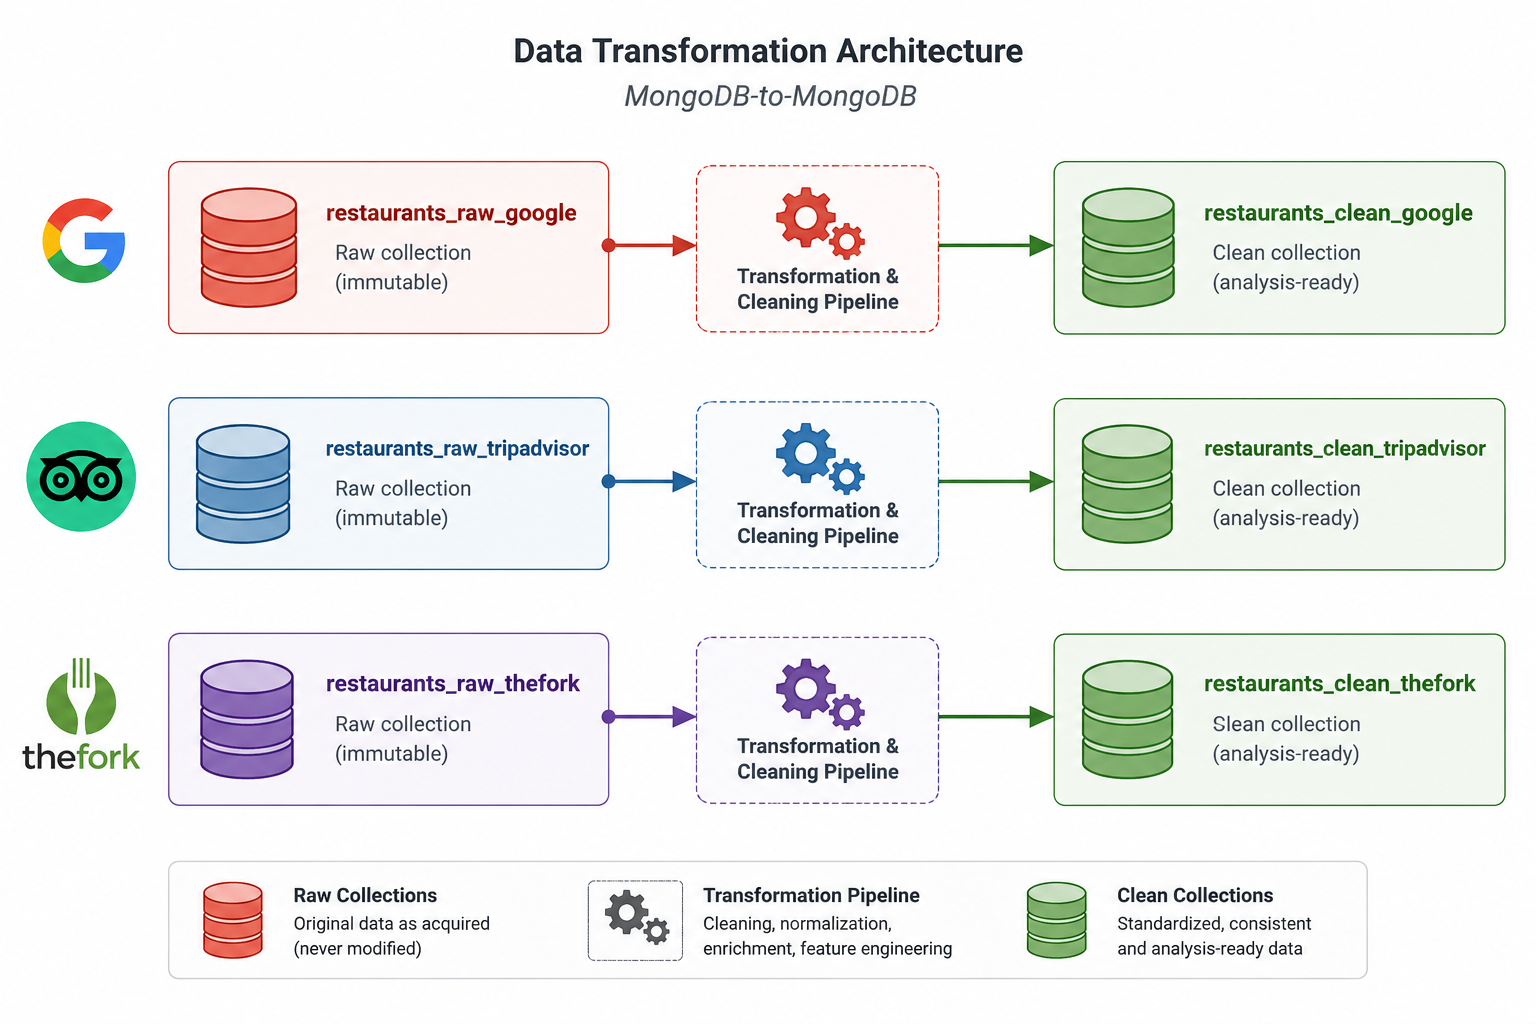
\includegraphics[width=\textwidth]{images/data_transformation_architecture.png}
\captionsetup{font=small}
\caption{MongoDB-to-MongoDB transformation architecture adopted in the project. Raw collections remain immutable and are transformed into dedicated clean collections through source-specific cleaning, normalization, and feature-engineering procedures.}
\label{fig:transformation_architecture}
\end{figure*}

\newcolumntype{Y}{>{\RaggedRight\arraybackslash}X}

\subsection{Clean Google Dataset Schema}

The \path|google_clean| transformation pipeline produces 10,786 clean records
in \collectionname{restaurants\_clean\_google}, obtained from 10,808 raw Google
records after removing 22 inert junk records. The goal of the cleaning step is
to keep only the fields needed for restaurant matching, quality control, and
cross-platform rating analysis. The subsequent integration stage further
restricts the Google anchor set to records classified as dining venues and
operational businesses. Table~\ref{tab:clean-google-schema} groups the fields
kept in the cleaned Google schema.

\begin{table*}[t]
\centering
\footnotesize
\setlength{\tabcolsep}{5pt}
\renewcommand{\arraystretch}{1.2}
\begin{tabularx}{\linewidth}{@{}p{0.25\linewidth}Y@{}}
\toprule
\textbf{Group} & \textbf{Cleaned information} \\
\midrule
Identity & Stable identifiers and display name, e.g. \texttt{\_id}, \texttt{place\_id}, \texttt{name}. \\
Location & Coordinates and structured address fields, e.g. latitude/longitude, street, house number, postal code, canonical city, province, and country. \\
Ratings & Google reputation data, including rating, review count, rating availability, and low-review indicator. \\
Classification & Google venue types transformed into higher-level categories such as restaurant, cafe/bar/bakery, non-dining, or unknown. \\
Quality flags & Operational and relevance checks, such as non-dining venue, non-operational business, geographic placeholder name, low review count, or out-of-area city. \\
Contact and price & Normalized website, phone number, price level, and parsed price range; also includes coverage indicators for website and phone availability. \\
Source richness & Compact evidence about the amount of Google information available, such as photo count and a slimmed sample of recent reviews. \\
Services and amenities & Optional Google service attributes, such as dine-in, takeout, delivery, reservations, outdoor seating, meal options, drinks, children-friendly service, pets, and restroom. \\
Metadata & Transformation timestamp and source collection name for traceability. \\
\bottomrule
\end{tabularx}
\caption{Grouped schema of the cleaned Google restaurant dataset.}
\label{tab:clean-google-schema}
\end{table*}

Examples of transformations include normalizing \path|formatted_address| into a
cleaner address field, extracting structured address components from Google
details, and standardizing city names such as \texttt{Milan} to
\texttt{Milano}. Ratings and review counts are taken from the detailed Google
response when available, with fallback to top-level raw values. Several fields
are created for data quality control rather than filtering records out
immediately. For example, \path|is_operational| is derived from Google business
status, \path|low_review| marks venues with few reviews, and the \texttt{flags}
array stores issues such as \path|non_dining|, \path|not_operational|, or
\path|city_out_of_area|. Contact fields are standardized to support
cross-platform matching. Websites are cleaned by removing URL schemes, leading
\texttt{www.}, and trailing slashes. Phone numbers are stripped of formatting
and converted to the Italian \texttt{+39} format when possible. The full raw
Google \texttt{details} object is not copied into the clean collection; only
selected useful fields are extracted, while the raw collection remains available
for audit and reproducibility.

\subsection{Clean Tripadvisor Dataset Schema}

The \path|tripadvisor_clean| transformation pipeline produces 7,539 clean
records in \collectionname{restaurants\_clean\_tripadvisor} and defines a
standardized schema for restaurant matching, quality control, and cross-platform
comparison. The cleaning step keeps only analytically useful information from
the raw Tripadvisor collection, while replacing raw semi-structured fields with
normalized, parsed, or derived attributes. In particular, raw fields such as
\path|price_range|, \path|cuisine_type|, \path|working_days_hours|,
\texttt{review}, \path|number_photo_uploaded|, and \path|phone_number| are not
copied directly into the clean collection; they are converted into structured
variables and remain available in the raw collection for audit purposes.
Table~\ref{tab:clean-tripadvisor-schema} summarizes the resulting grouped
schema.

\begin{table*}[t]
\centering
\footnotesize
\setlength{\tabcolsep}{5pt}
\renewcommand{\arraystretch}{1.2}
\begin{tabularx}{\linewidth}{@{}p{0.25\linewidth}Y@{}}
\toprule
\textbf{Group} & \textbf{Cleaned information} \\
\midrule
Identity & Stable identifiers and source references, such as \texttt{\_id}, \texttt{source\_url}, \texttt{ta\_location\_id}, and \texttt{restaurant\_name}. \\
Location & Normalized address information, including \texttt{address}, \texttt{street}, \texttt{house\_number}, \texttt{postal\_code}, \texttt{city}, and address coverage flags. Coordinates are included as \texttt{latitude} and \texttt{longitude} after Nominatim geocoding. \\
Ratings & Tripadvisor reputation variables, including \texttt{rating}, \texttt{total\_review}, rating and review-count availability indicators, and the \texttt{low\_review} flag. \\
Price and cuisine & Parsed price information through \texttt{price\_band} and \texttt{price\_tier\_level}, together with normalized cuisine categories stored in \texttt{cuisines}. \\
Source richness & Compact indicators of source completeness, including \texttt{photo\_count}, structured \texttt{opening\_hours}, \texttt{has\_hours}, review samples, \texttt{sample\_size}, and \texttt{has\_reviews}. \\
Contacts & Standardized contact fields, including cleaned \texttt{website}, normalized \texttt{phone}, \texttt{email}, and the corresponding coverage indicators. \\
Quality flags & A consolidated \texttt{flags} array storing data quality issues such as \texttt{no\_rating}, \texttt{missing\_review\_count}, \texttt{low\_review}, \texttt{missing\_address}, \texttt{missing\_coordinates}, \texttt{no\_reviews}, or \texttt{no\_hours}. \\
Metadata & Transformation timestamp and source collection name, stored in \texttt{\_transformed\_at} and \texttt{\_source\_collection}, for reproducibility and traceability. \\
\bottomrule
\end{tabularx}
\caption{Grouped schema of the cleaned Tripadvisor restaurant dataset.}
\label{tab:clean-tripadvisor-schema}
\end{table*}

The transformation pipeline standardizes fields that are originally inconsistent or difficult to use directly. Restaurant names are cleaned by collapsing whitespace, while the Tripadvisor location identifier is extracted from the restaurant URL and used as a stable source-specific key. Address strings are normalized and parsed into street, house number, postal code, and city components, with \texttt{has\_address} marking address availability. Since Tripadvisor does not provide coordinates in the raw scrape, the cleaned address is geocoded through Nominatim/OpenStreetMap as part of the transformation stage~\cite{osm-nominatim}. In the final pipeline, Tripadvisor coordinate coverage reaches 84.0\%, and the post-integration assessment reports a median geocoding error of 10.1 m on gold-standard matched rows. Ratings are parsed from Tripadvisor's comma-decimal format, review counts are converted from raw textual values into integers, and coverage indicators are added to distinguish missing information from valid low values. Price ranges are validated and converted into both a source price band and an ordinal tier, while cuisine strings are split, trimmed, and de-duplicated into a list. Opening hours are transformed from raw text into structured daily time intervals, preserving split shifts when present. Review data is reduced to a compact sample containing only selected fields, such as nickname, title, text, date, and contribution count. Contact fields are normalized for matching purposes: websites are stripped of schemes, leading \texttt{www.}, and trailing slashes, while Italian phone numbers are converted to a canonical \texttt{+39} format when possible. The clean collection therefore avoids copying bulky or redundant raw fields, but preserves the raw Tripadvisor collection as the audit trail for reproducibility.


\subsection{Clean TheFork Dataset Schema}

The \path|thefork_clean| transformation pipeline produces 1,344 clean records
in \collectionname{restaurants\_clean\_thefork} and provides a standardized
representation of restaurant information for entity matching, data quality
assessment, and integration with other restaurant platforms. The cleaning
process preserves the most relevant source information while replacing raw or
semi-structured attributes with normalized and analytically usable features. In
particular, raw fields such as \path|price_range|, \texttt{discount},
\path|cuisine_type|, \path|working_days_hours|, and the original nested review
structure are transformed into standardized variables, while the raw collection
remains available as an audit trail. Table~\ref{tab:clean-thefork-schema}
summarizes the corresponding clean TheFork schema.

\begin{table*}[t]
\centering
\footnotesize
\setlength{\tabcolsep}{5pt}
\renewcommand{\arraystretch}{1.2}
\begin{tabularx}{\linewidth}{@{}p{0.25\linewidth}Y@{}}
\toprule
\textbf{Group} & \textbf{Cleaned information} \\
\midrule
Identity & Stable identifiers and source references, including \texttt{\_id}, \texttt{source\_id}, \texttt{tf\_id}, \texttt{restaurant\_url}, and \texttt{restaurant\_name}. \\
Location & Native TheFork coordinates and normalized address information, including \texttt{latitude}, \texttt{longitude}, \texttt{address}, \texttt{street}, \texttt{house\_number}, \texttt{postal\_code}, and canonical city names. \\
Ratings & TheFork reputation metrics, including \texttt{rating}, \texttt{review\_count}, coverage indicators, and the \texttt{low\_review} quality flag. \\
Price and promotions & Structured economic information through \texttt{avg\_price\_eur}, parsed promotional discounts (\texttt{discount\_pct}), and discount availability indicators. \\
Cuisine & Normalized cuisine categories stored in \texttt{cuisines} together with extracted dietary tags such as vegetarian, vegan, halal, kosher, and gluten-free options. \\
Opening hours & Structured opening schedules represented as daily opening and closing intervals, together with availability indicators. \\
Source richness & Additional information describing source completeness, including \texttt{photo\_count} and review snippets. \\
Review sample & Slimmed review objects, sample statistics, review coverage indicators, and consistency checks between platform ratings and review-sample ratings. \\
Quality flags & Data quality indicators such as \texttt{no\_rating}, \texttt{missing\_review\_count}, \texttt{low\_review}, \texttt{rating\_sample\_divergent}, and \texttt{invalid\_cuisine\_type}. \\
Metadata & Transformation timestamp, source collection information, and scraping provenance attributes. \\
\bottomrule
\end{tabularx}
\caption{Grouped schema of the cleaned TheFork restaurant dataset.}
\label{tab:clean-thefork-schema}
\end{table*}

The transformation pipeline standardizes restaurant names and addresses, extracts a stable TheFork venue identifier from the source key, and canonicalizes location information for consistent matching across platforms. Unlike Tripadvisor, TheFork already provides native geographic coordinates, which are preserved without additional geocoding. Ratings and review counts are validated and converted into numeric variables, while coverage indicators are introduced to distinguish missing information from valid values. Price information is transformed into a numeric average price expressed in euros, and promotional offers are parsed into structured discount percentages whenever possible. Cuisine information is cleaned, de-duplicated, and separated from dietary or religious attributes, which are mapped to standardized tags. Opening hours are converted into structured daily intervals, preserving complex schedules and overnight closures. Review data is reduced to compact review objects containing only the most relevant information, while additional features such as \texttt{sample\_avg\_rating} and \texttt{rating\_sample\_divergent} are generated to support quality assessment. The resulting dataset therefore provides a compact, consistent, and analysis-ready representation of TheFork restaurants while preserving the raw collection for reproducibility and auditing purposes.



\section{Schema Matching}

The objective of the schema matching phase is to identify the semantic correspondences between the clean schemas generated from Google Places, Tripadvisor and TheFork. Unlike entity resolution, which operates at the record level, schema matching focuses on the structural and conceptual alignment of attributes across data sources. The outcome of this phase is a formal set of correspondences and conflict-resolution rules that provide the foundation for the subsequent integration process.

The analysis used the three clean transformation outputs documented above:
Google, Tripadvisor, and TheFork.
Since each platform models restaurant information according to its own schema
and business objectives, direct integration is not possible without first
identifying which attributes describe the same real-world concept and which
representation conflicts must be resolved.

Schema matching was performed according to two complementary perspectives. The first concerns the semantic relationship between attributes, while the second concerns the representation conflicts that emerge when equivalent concepts are modeled differently. Following the classical schema integration literature~\cite{rahm-bernstein-2001}, four types of semantic correspondences were considered:


\begin{itemize}
\item \textbf{Equivalence} ($\equiv$), when two attributes represent the same real-world property;
\item \textbf{IS-A} ($\sqsubseteq$), when one attribute represents a specialization of a broader concept;
\item \textbf{Overlap} ($\sqcap$), when two attributes partially intersect but neither subsumes the other;
\item \textbf{Disjointness} ($\bot$), when two attributes appear similar but actually describe different facts and therefore must never be merged.
\end{itemize}

The matching process revealed that most restaurant descriptors are semantically equivalent across the three platforms. Restaurant names, addresses, postal codes, cities, ratings, review counts, coordinates, opening hours, and contact information all describe the same underlying concepts, although they are often represented using different structures, naming conventions, or measurement scales. Table~\ref{tab:schema-matching-correspondences} gives representative correspondences.

\begin{table*}[t]
\centering
\footnotesize
\setlength{\tabcolsep}{4pt}
\begin{tabularx}{\linewidth}{@{}
>{\RaggedRight\arraybackslash}p{0.27\linewidth}
>{\RaggedRight\arraybackslash}p{0.19\linewidth}
>{\RaggedRight\arraybackslash}X
@{}}
\toprule
\textbf{Integrated Concept} & \textbf{Relation} & \textbf{Source Attributes} \\
\midrule
Restaurant name & $\equiv$ Equivalence & \texttt{name}, \texttt{restaurant\_name} \\
Address information & $\equiv$ Equivalence & \texttt{address}, \texttt{street}, \texttt{postal\_code}, \texttt{city} \\
Geographic coordinates & $\equiv$ Equivalence & \texttt{latitude}, \texttt{longitude} \\
Restaurant rating & $\equiv$ Equivalence & \texttt{rating} \\
Review count & $\equiv$ Equivalence & \texttt{review\_count}, \texttt{total\_review} \\
Dietary information & $\sqsubseteq$ IS-A & \texttt{dietary\_options}, \texttt{serves\_vegetarian\_food} \\
Cuisine descriptors & $\sqcap$ Overlap & \texttt{cuisines}, \texttt{primary\_type} \\
Platform identifiers &
$\bot$ Disjointness &
\texttt{place\_id}, \texttt{ta\_location\_id}, \texttt{tf\_id}
\\
\bottomrule
\end{tabularx}
\caption{Examples of semantic correspondences identified during schema matching.}
\label{tab:schema-matching-correspondences}
\end{table*}

Several representation conflicts were also identified. The most important concerns restaurant ratings. Google Places and Tripadvisor use a 1--5 scale, whereas TheFork adopts a 0--10 scale. Although the three attributes describe the same concept, direct comparison would be misleading without normalization. This represents a scaling conflict rather than a semantic discrepancy. Similarly, price information is represented using heterogeneous formats, including categorical price levels, symbolic price bands, and explicit average prices expressed in euros. Cuisine descriptors are an additional semantic conflict, since the three platforms use different and even cross-language vocabularies; this overlap is resolved later through an explicit canonical cuisine taxonomy applied during dataset integration (Section~\ref{sec:cuisine-reconciliation}).

Additional conflicts arise from structural differences. Address information may be represented either as a single normalized string or as a set of decomposed components. Review data exhibit even greater heterogeneity, since each platform provides different review structures, metadata, and levels of detail. Consequently, review objects are preserved together with their source provenance rather than being merged directly. Table~\ref{tab:schema-matching-conflicts} summarizes the main conflict types and their resolution strategies.

\begin{table*}[t]
\centering
\footnotesize
\begin{tabular}{p{0.25\linewidth}p{0.25\linewidth}p{0.38\linewidth}}
\toprule
\textbf{Conflict Type} & \textbf{Example} & \textbf{Resolution Strategy} \\
\midrule
Naming conflict & \texttt{name} vs \texttt{restaurant\_name} & Canonical attribute naming \\
Scaling conflict & Ratings 1--5 vs 0--10 & Rating normalization \\
Structural conflict & Address strings vs structured components & Schema harmonization \\
Semantic conflict & Regional vs national cuisine labels & Vocabulary mapping \\
Coverage conflict & Missing coordinates in Tripadvisor & Geocoding and enrichment \\
\bottomrule
\end{tabular}
\caption{Main conflicts identified during schema matching.}
\label{tab:schema-matching-conflicts}
\end{table*}

A particularly important outcome of the analysis concerns source-specific identifiers. Google Places, Tripadvisor, and TheFork provide stable identifiers within their own platforms, namely \texttt{place\_id}, \texttt{ta\_location\_id}, and \texttt{tf\_id}. Although these identifiers uniquely identify restaurants within each source, they belong to independent namespaces and therefore cannot be used as integration keys. Entity resolution must consequently rely on descriptive attributes such as restaurant names, addresses, coordinates, and contact information.

The correspondences are not only descriptive: they determine the actual integrated schema. Google identity and coordinates are used as the canonical restaurant backbone; TheFork's native 0--10 rating is normalized into a comparable \texttt{thefork\_rating\_5}; Google, Tripadvisor, and TheFork ratings are intentionally preserved as separate attributes because rating disagreement is the object of analysis; price signals from Google price levels, Tripadvisor price bands, and TheFork average prices are mapped to a common price representation; and review objects are not fused into a single text field because their structures, sampling rules, and provenance differ across platforms. The schema matching phase therefore establishes the semantic foundation required for integration. By explicitly defining attribute correspondences, identifying representation conflicts, and documenting source-specific characteristics, it becomes possible to generate consistent mapping rules and construct a unified restaurant schema without ambiguity or loss of information.
